\chapter{Project Preparations}\label{ch:project_prep}
The first phase of this thesis consisted mostly of many attempts at getting a working environment set up on a Linux machine, running ROS.
The main goal was to be able to allow depth cameras to communicate with ROS 2 and control simple devices through this system.
ROS was chosen as the platform to control devices as it is already used by many of the devices set up in the lab and robots on the university campus.
The lab also had Microsoft's Kinect v2 depth cameras already accessible and was known to have previously been successfully set up and used with ROS so this became the sensor of choice.

While this all seemed simple in theory, with previous work at the university proving that the proposed work was possible, in reality, the Kinect v2 integration with ROS was not regularly maintained and ROS had a new major version release in this period, so it required a significant amount of work to get the device to communicate with a ROS 2 distribution.

\section{Progress and Roadblocks}

The first step was to get a ROS 2 distribution running on the machine and learn the inner workings of the operating system.
The ROS website and documentation suggest that an installation on a Windows machine is possible and is supported but the overwhelming response from members of their community and in their forums was that the Windows installation was not an easy task and often performed worse.
The consensus was that a Linux installation was the most reliable and safest option.
This was the first of many times that the environment setup had to pivot and try some alternative method.

Running ROS 2 on Windows Subsystem for Linux (WSL) felt like the next logical step as this would allow ROS 2 to run on a Linux installation without a significant change to the machine that this was being run on.
It was quickly discovered that WSL would not be a suitable operating environment as the visual tools of ROS would still be required for debugging and testing.
Soon after, a successful installation of ROS on native Windows was achieved but with very little documentation or support from the community, it was clear that this was not the best option and was only really suitable for small, simple deployments.

This then led to a pivot to running Linux on a virtual machine within Windows.
Using the Linux distribution (distro) Ubuntu 22.04, Jammy Jellyfish, was the first environment setup where the ROS 2 distribution Humble Hawksbill was installed and ran smoothly, with tools like RViz and the built-in turtle simulator working as expected.
After getting ROS running, and also throughout the remainder of the setup process, there was a significant amount of time spent learning the ROS environment and how to use the tools provided with it, including sending messages between node topics and creating custom messages and services.
This was both in the terminal commands and through the Python client library for ROS.

The next step was to get the Kinect to communicate with ROS 2.
To do so, the Kinect needed to communicate with the virtual machine (VM) through USB passthrough.
Out of the box, VirtualBox, the VM software used to run the Linux distro, only supports USB 1.0 and USB 2.0 devices, while the Kinect requires a USB 3.0 connection to send the large amount of data that it captures.
Installing Oracle's VirtualBox Extension Pack allows USB 3.0 devices to connect to the VM through the host machine, however, it was later discovered that the Kinect v2 drivers for Linux do not support connection through a virtual machine.

Again, this meant pivoting to a new environment setup and dual-booting the machine to run Linux natively.
This way it was possible to get OpenKinect's Libfreenect2 drivers for the Kinect v2 working and it was now possible to capture colour and depth data from the sensors using software provided with the drivers.

It was soon realised that there is no existing integration for the Kinect v2 with ROS 2 as the hardware at a decade old is now slightly outdated, having been succeeded four years ago by the Azure Kinect DK.
Since this was the only depth camera available on hand, it was decided that the best course of action would be to attempt to get the Kinect working on the known solution of ROS 1 and then use the ROS Bridge to forward the data to ROS 2.
Using the most recent version of ROS 1, Noetic Ninjemys, the Kinect was able to send depth and colour data to ROS at several resolutions using a fork of the Kinect bridge from the Institute of Artificial Intelligence at the University of Bremen (IAI), that supported OpenCV 4.0, an open source computer vision library.

Open Robotics provides a bridge between ROS 1 and ROS 2 that allows for communication between the two systems and translation of the topics, services, and actions between nodes in either direction.
Using ROS Humble, ROS Noetic and the ROS 1 bridge, it was possible to send data between nodes in ROS 1 and ROS 2 across the bridge.
When using the Kinect bridge at the same time, there were struggles getting all parts of the system to work stably and consistently.
There appeared to be much more documentation and support for a setup using a previous distribution of ROS2, Foxy Fitzroy so this was the next change needed to be made for the project.

Unfortunately, ROS Foxy does not run on Ubuntu 22.04, so the distro had to be downgraded to Ubuntu 20.04, Focal Fossa.
This was the final roadblock encountered in preparations trying to get the Kinect working with ROS 2.
On Ubuntu 20.04, with ROS Foxy, ROS Noetic, Libfreenect2, the IAI Kinect Bridge, and the ROS 1 bridge, it was finally possible to read colour and depth data from the Kinect into ROS 2 and into Python using the ROS Client Python library.

This leads to a rather convoluted setup to allow communication as shown in Figure~\ref{fig:kinect_ros}.

\begin{figure}[!htb]
    \caption{Kinect to ROS 2 Layers}
    \makebox[\textwidth][c]{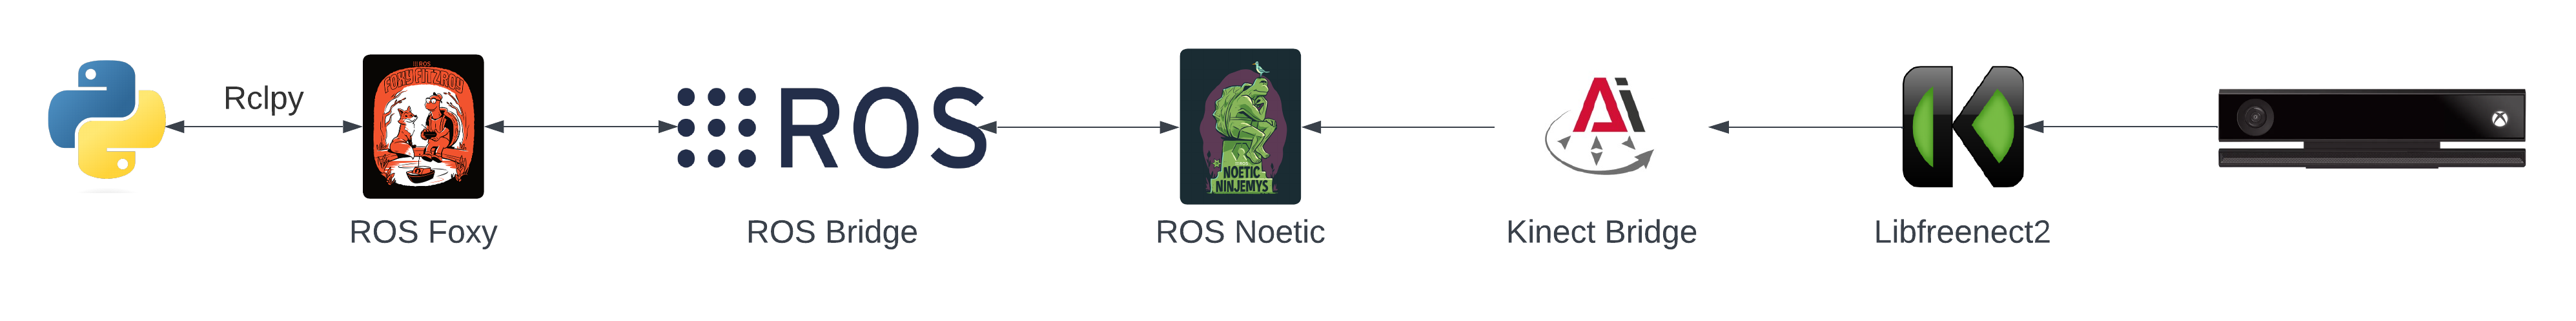
\includegraphics[width=0.9\pdfpagewidth]{ROS Kinect Layers.png}}
    \label{fig:kinect_ros}
\end{figure}

The Kinect data can be read using the Libfreenect2 drivers from Open Kinect.
This is then sent via the IAI Kinect Bridge to ROS 1.
Using the ROS 1 bridge, the data is then sent to ROS 2 where it can finally be read by the ROS Client Python library and more meaningful operations can be done with it.

\section{Technology Stack}
Using this setup for ROS and the Kinect, the final proposed tech stack for continuing development is shown in Figure~\ref{fig:tech_stack}.

The setup outlined previously will run on an Ubuntu machine within the home and connect to a Kinect v2 depth camera.
External smart home devices will be controllable through ROS Foxy either via data from the Kinect or through scripts written in Python.
Additionally, there will be a TypeScript front-end provided as well that will be accessible within the network to allow users to control devices manually.
This is because any smart home system should only ever add functionality to a home, never replace existing functionality.
There should always be the option to control the devices manually.
The web interface will also allow users to add new gestures to be recognised by the Kinect and to control devices in new ways.
Users of the environment will be able to interact with both the front-end and with the Kinect, via movement and gestures, to control devices in the home.

\begin{figure}[H]
    \caption{Proposed Technology Stack}
    \makebox[\textwidth][c]{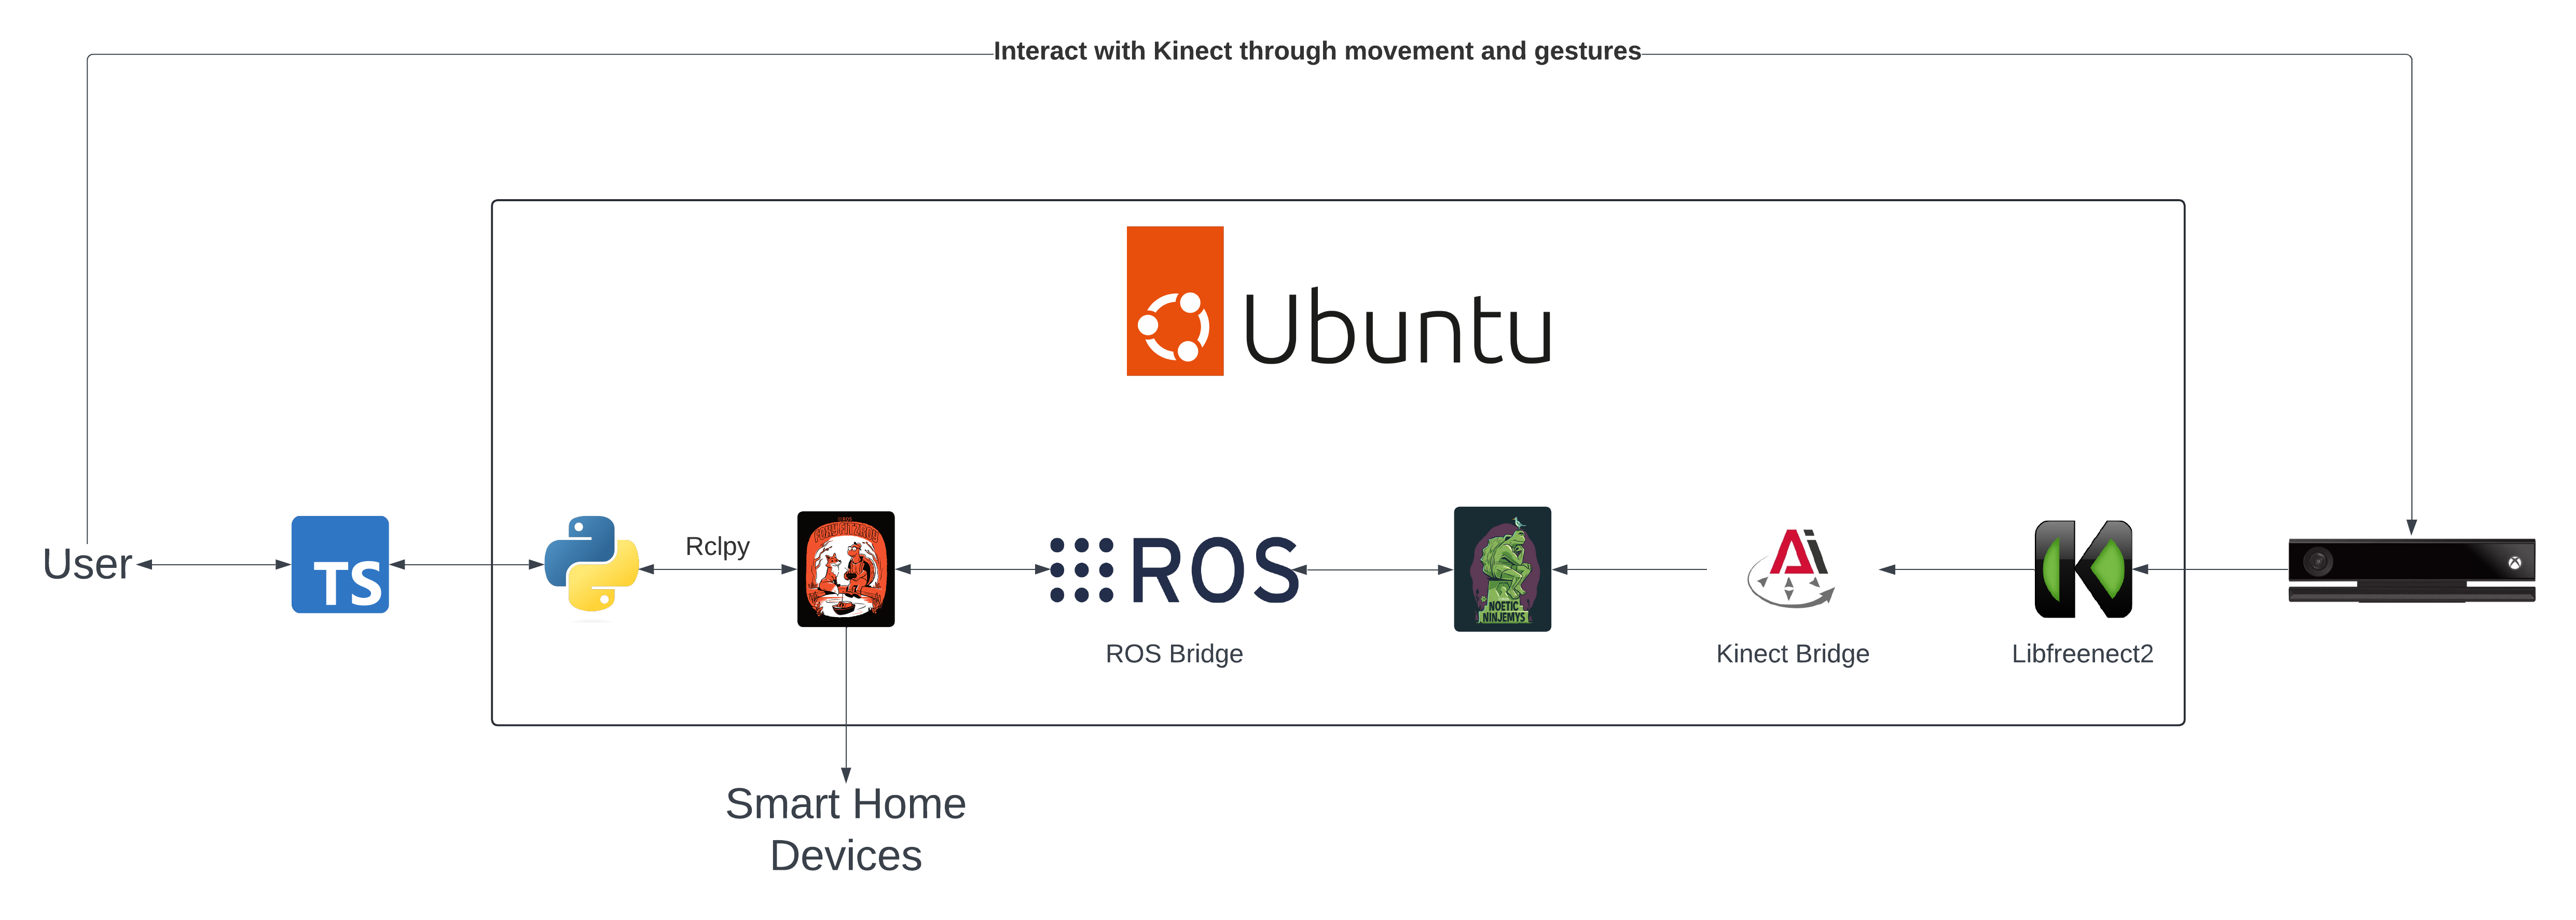
\includegraphics[width=\textheight,angle=-90]{Tech Stack.png}}
    \label{fig:tech_stack}
\end{figure}

\newpage

\section{Preliminary Results}

After the ROS environment was set up, a couple of demonstration programs were written in Python to test the functionality and as a proof of concept, to show that external devices could be controlled.

The first was a simple program that extracted depth data from the Kinect and displayed this in the terminal in the form of American Standard Code for Information Interchange (ASCII) art.
This is achievable by taking a scale of the depth data and mapping this to a range of characters of increasing density of pixels.
The more pixel-dense characters represent objects that are closer to the sensor and less dense characters represent objects that are further away.
As shown in Figure~\ref{fig:depth_ascii}, this is a simple way to visualise the depth data that the Kinect is capturing as the user's outline is visible in the ASCII art image.

\begin{figure}[!htb]
    \caption{Depth Data as ASCII Art in the Terminal}
    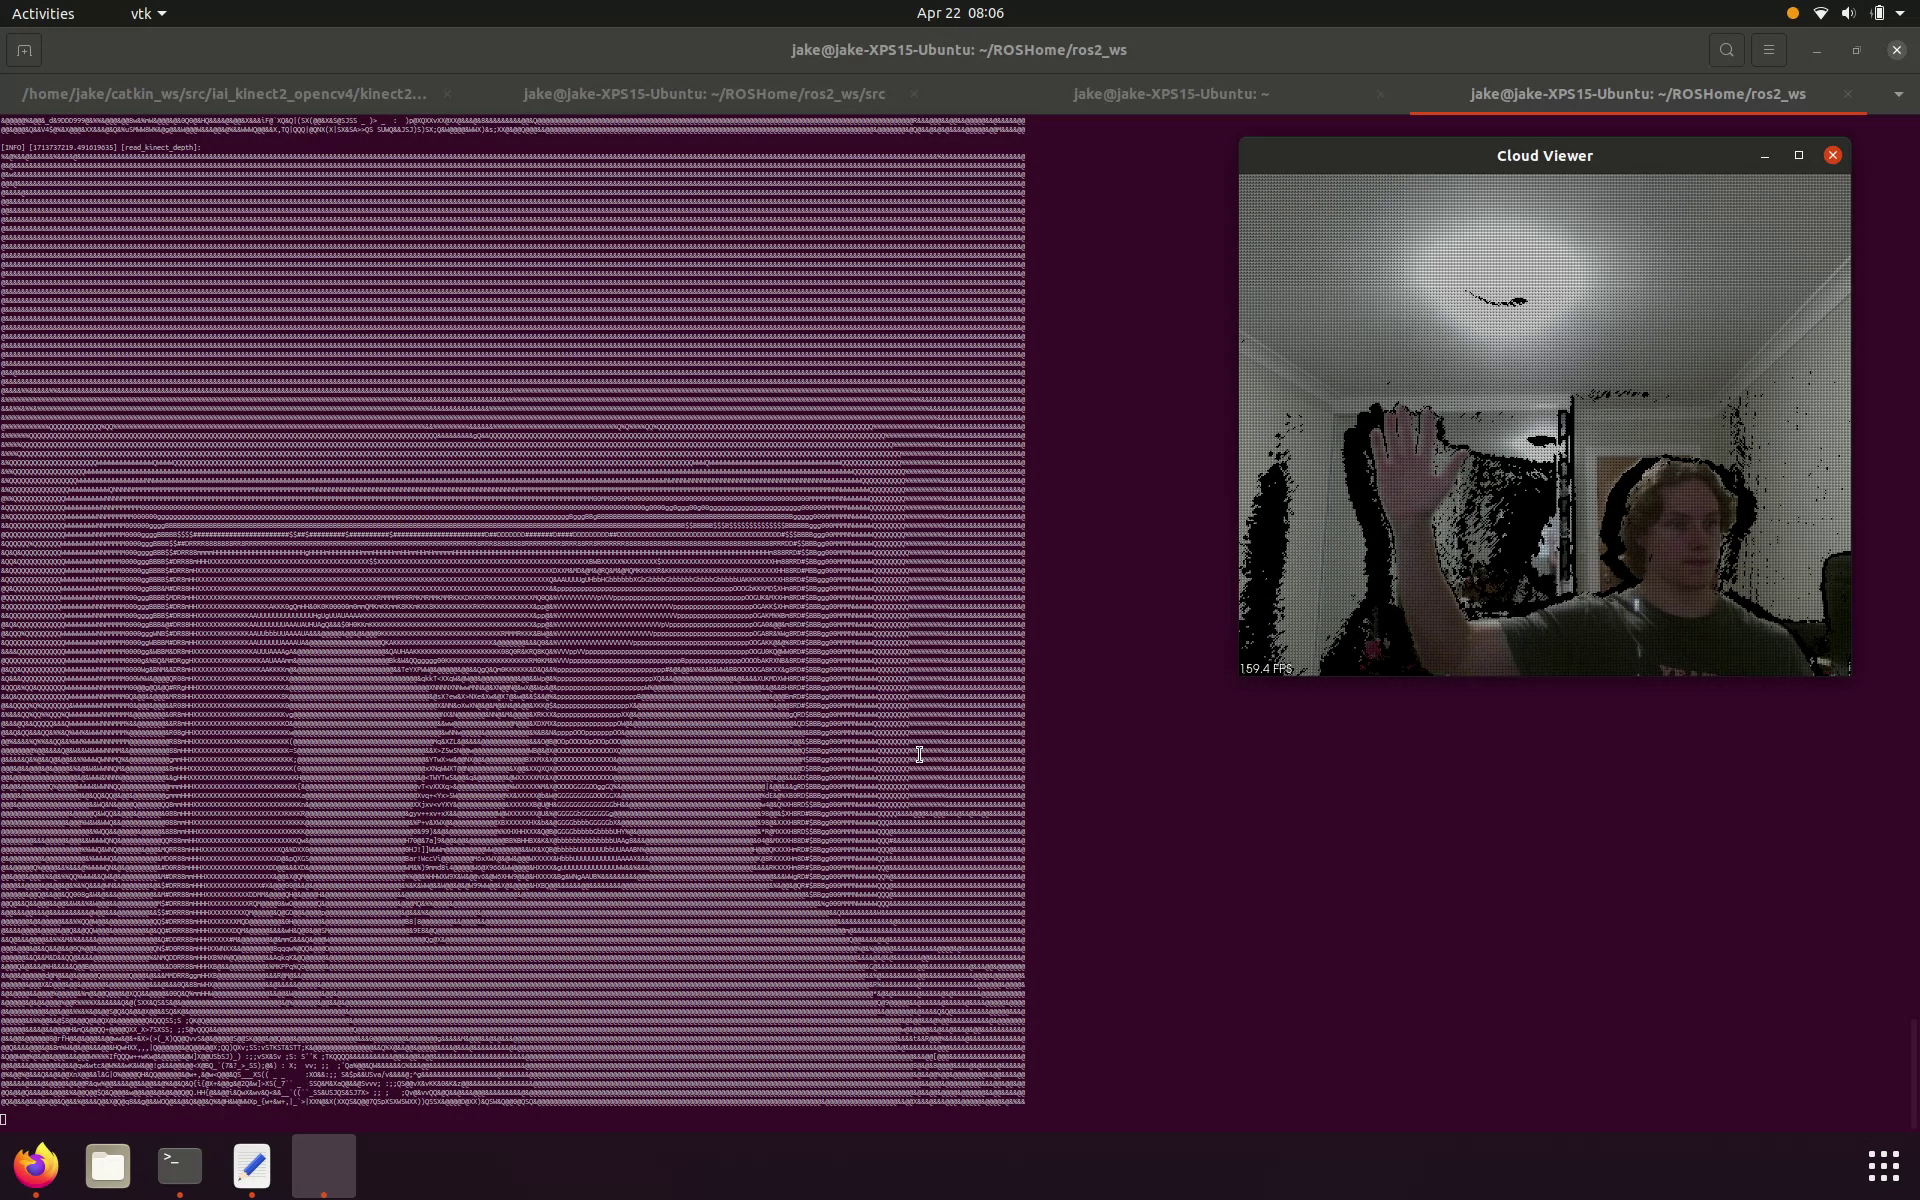
\includegraphics[width=\textwidth]{Depth Data Demo.png}
    \small
    On the right of the image is the provided Kinect viewer tool showing a live feed from the camera, and on the left is the ASCII art representation of the depth data in the terminal.
    \label{fig:depth_ascii}
\end{figure}

The second program extracted the colour data from the camera and also printed this to the terminal by using space characters (`` '') with its background colour set to the colour of the pixel in the camera.
The resolution of the image had to be decreased in order to fit the entire image on the terminal screen, so an average colour of surrounding pixels was taken.
As shown in Figure~\ref{fig:colour_image}, the colour data was able to be displayed in the terminal in real-time as read from the Kinect camera.

\begin{figure}[!htb]
    \caption{Colour Data as an Image in the Terminal}
    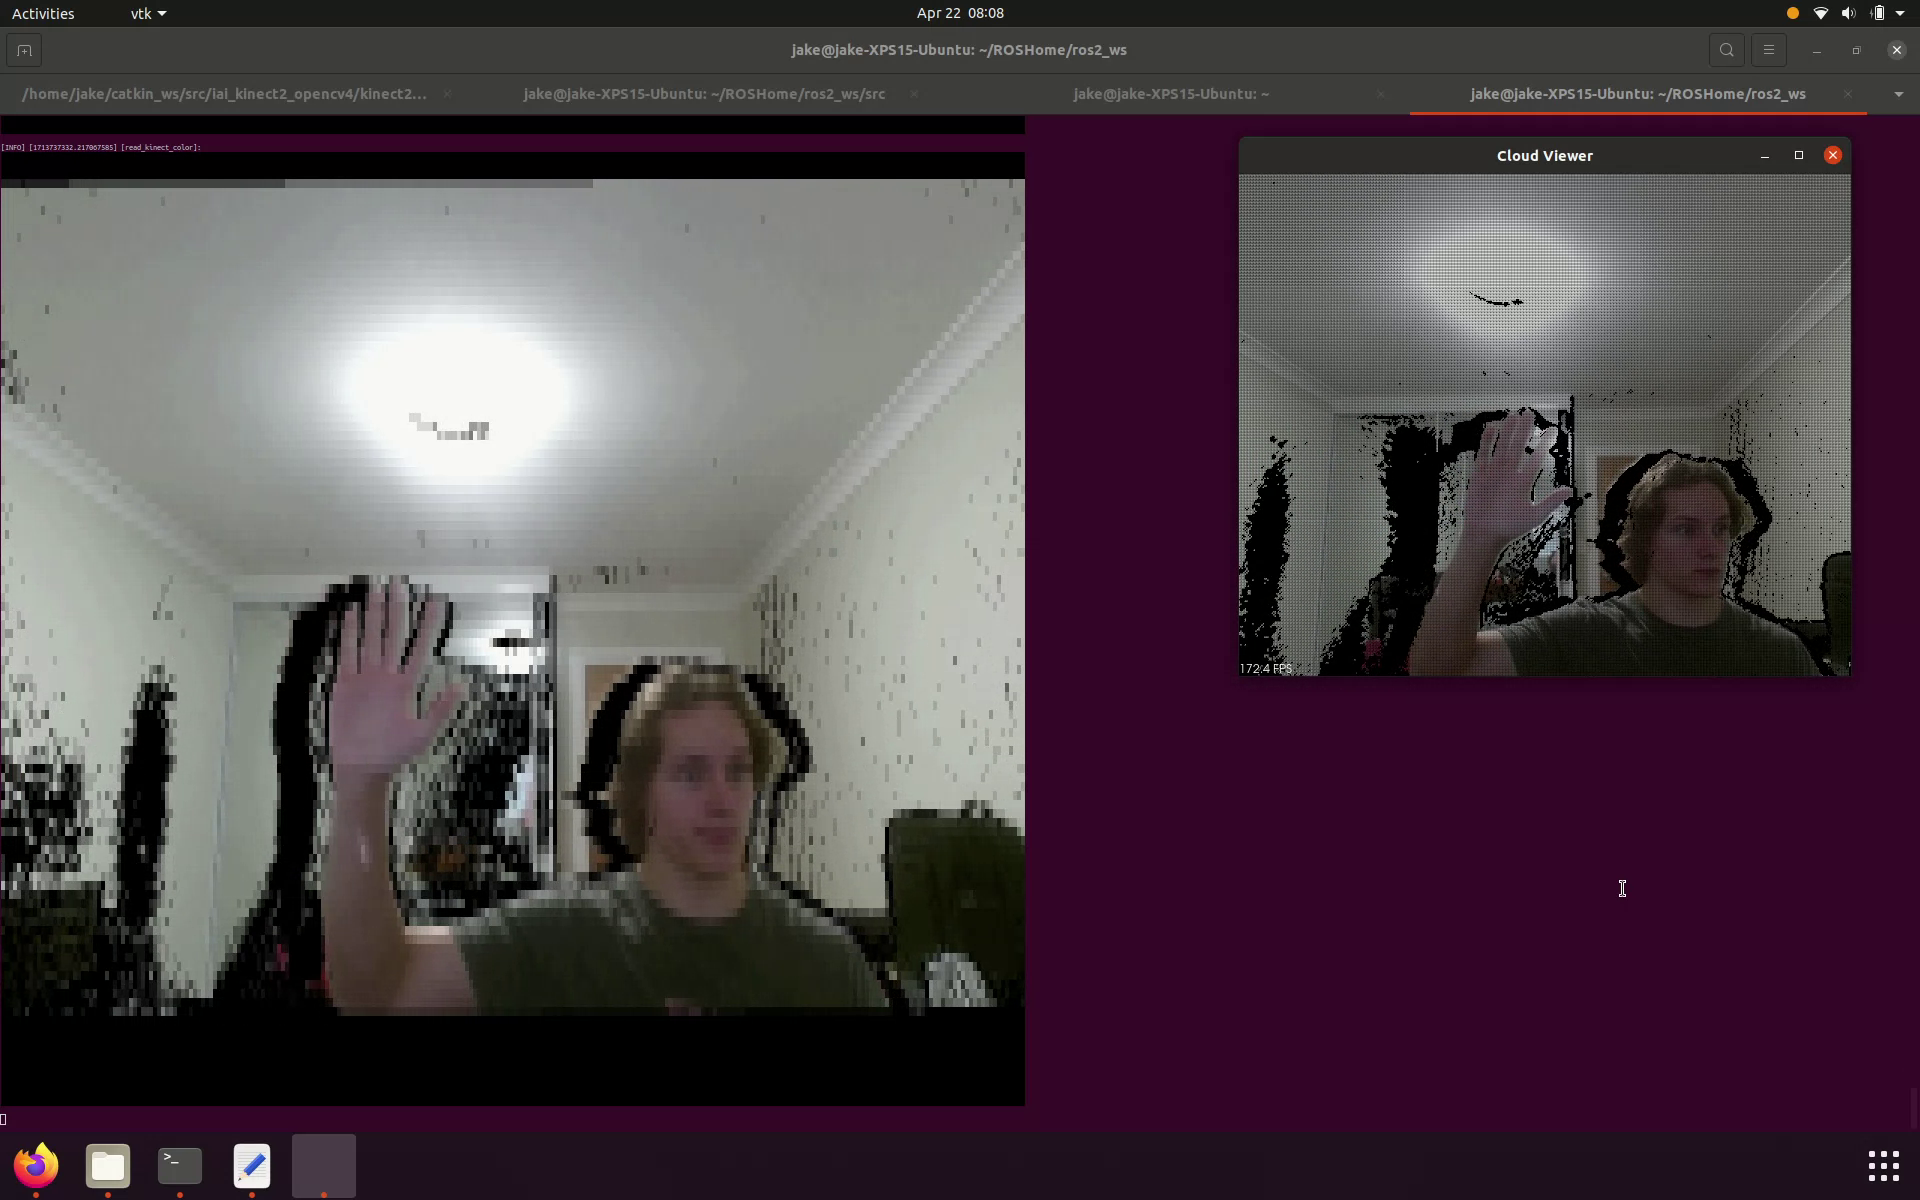
\includegraphics[width=\textwidth]{Colour Data Demo.png}
    \small
    On the right of the image is the provided Kinect viewer tool showing a live feed from the camera, and on the left is the colour data printed as coloured space characters in the terminal.
    \label{fig:colour_image}
\end{figure}

These first demonstrations were initially only implemented for the sake of testing to ensure that the Kinect was working as expected and that both the depth and colour data could be read from the camera.
The third and final demonstration was a simple program that allowed the user to control a turtle in the ROS turtle simulator using hand gestures.

By moving both hands in front of the Kinect, the user could move the turtle forwards, backwards, or stationary and turn the turtle left, right or stationary.
The direction the turtle moved was dependent on the distance of the closest hand to the camera and the direction the turtle moved was dependent on the difference in the distances of the two hands to the camera.

\textbf{Movement Controls:}\newline
If the user's closest hand was closer than 200mm to the camera, the turtle would move forwards.\newline
If the user's closest hand was further than 500mm from the camera, the turtle would move backwards.\newline
If the user's closest hand was between these two distances, the turtle would remain stationary.

\textbf{Rotation Controls:}\newline
If the user's left hand was more than 200mm further from the camera than the right hand, the turtle would turn left.\newline
If the user's right hand was more than 200mm further from the camera than the left hand, the turtle would turn right.\newline
If the difference in distance between the two hands was less than 200mm, the turtles would not turn.

This can be observed in Figure~\ref{fig:turtle_fwd} and Figure~\ref{fig:turtle_turn} where the turtle is moving forwards as the user's hands are close to the camera and the turtle is turning left as the user's left hand is further from the camera than the right hand.

\begin{figure}[!htb]
    \caption{Turtle Simulation: Moving Forwards}
    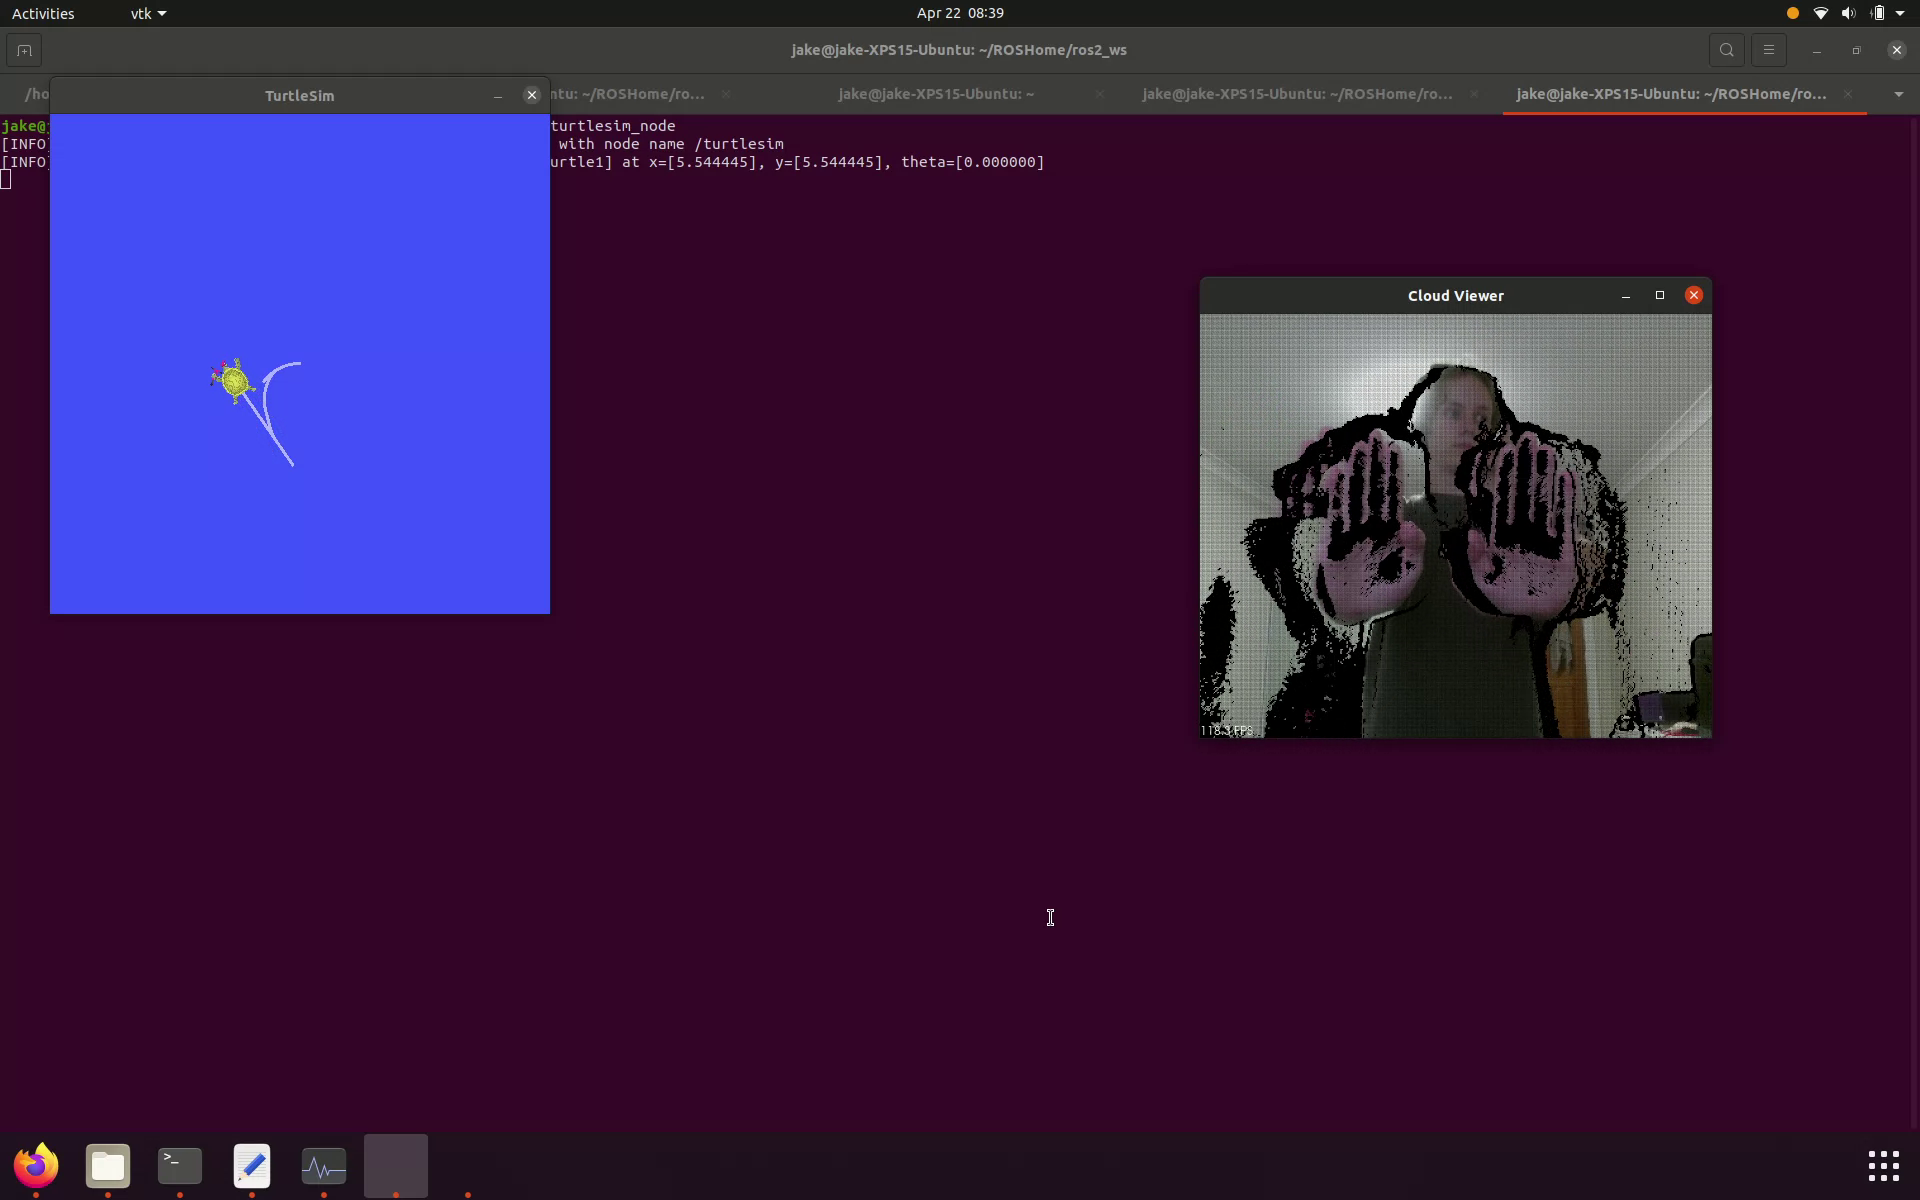
\includegraphics[width=\textwidth]{Gesture Control Demo Forwards.png}
    \small
    The user's hands are closer than 200mm to the camera so the turtle is moving forwards.
    \label{fig:turtle_fwd}
\end{figure}

\begin{figure}[!htb]
    \caption{Turtle Simulation: Turning Left and Reversing}
    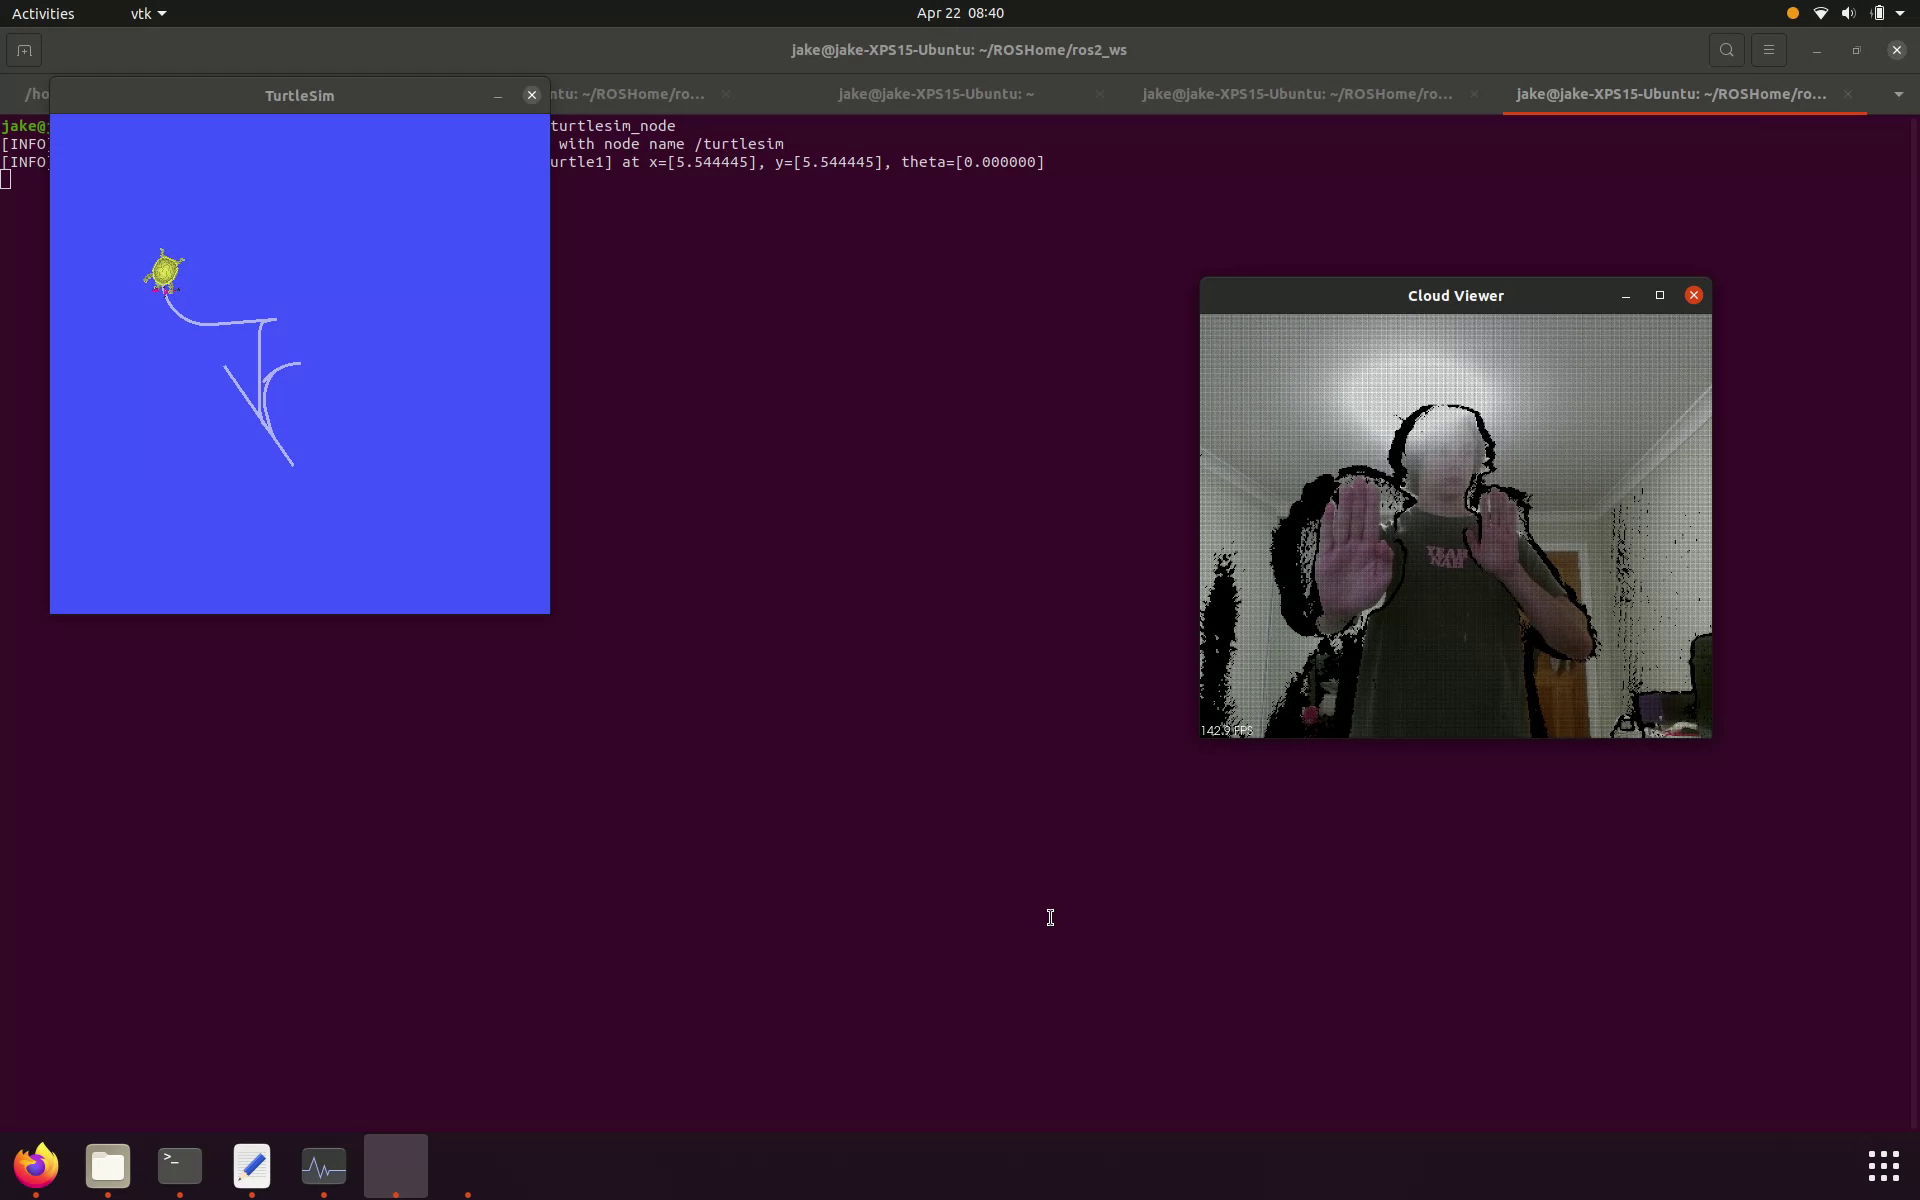
\includegraphics[width=\textwidth]{Gesture Control Demo Turning.png}
    \small
    The user's hands are further than 500mm from the camera and their left hand is more than 200mm further from the camera than their right hand so the turtle is moving backwards and turning left.
    \label{fig:turtle_turn}
\end{figure}

This system, however, did not actually use any hand gesture recognition, it simply measured the distance of the closest object on the left and the right half of the Kinect's sensor.
Despite this program's primitive control methods, this demonstration was a proof of concept, showing that the Kinect could be used to control external devices through ROS and that the system was viable for further development.